\chapter{Unit Tests}
Zur frühzeitigen Erkennung von Fehlern und der Sicherung der Qualität der Software wurden für das Projekt einige Unit Tests implementiert. Diese beschränken sich im Wesentlichen jedoch auf die Applikationssicht der Software, da dort der größte Teil der tatsächlichen Businesslogik implementiert ist. 

Für die Peripherie der Software wurde zunächst auf Unit Tests verzichtet, da dieser Teil des Programms ohnehin leicht und häufig austauschbar sein soll und daher von geringerer Wichtigkeit ist, sodass ihm auch beim Testen eine geringere Priorität beigemessen wurde. Lediglich in der Adapterschicht wird eine Klasse, der \code{OpinionMapper} getestet. Auch für den Domaincode wurde zunächst auf Unit Tests verzichtet, da sich die dort implementierte Businesslogik hauptsächlich auf die Definition von Klassen und ihre Attribute beschränkt, es existieren jedoch keine Methoden, welche tatsächlich komplexere Logik enthalten.

\section{ATRIP-Regeln}
Bei den ATRIP-Regeln handelt es sich um fünf grundlegende Regeln für die Erstellung guter Unit Tests. Inwiefern diese für das vorliegende Projekt eingehalten wurden, wird in den nachfolgen Abschnitten aufgezeigt.

\paragraph{Automatic} Alle implementierten Unit Tests laufen vollständig eigenständig ab, da keinerlei manuelle Eingriffe, etwa in Form von Werteeingaben, notwendig sind. Außerdem überprüfen alle Tests ihre Ergebnisse durch Assertions automatisch.

\paragraph{Thorough} Da es sich bei dieser Regel um eine \enquote{weiche} Regel handelt, ist eine eindeutige Entscheidung, ob alles Notwendige getestet wurde und damit die Regel erfüllt ist schwierig. Als \enquote{notwendig} wurde für das vorliegende Projekt die wesentliche Businesslogik und damit die Applikationsschicht definiert. Diese wird mit einer hohen Code-Coverage getestet, sodass die implementierten Tests durchaus als gründlich bezeichnet werden können. (vgl. \autoref{sec:code-coverage}) Es wurden allerdings keine Tests für spezifische Softwarefehler implementiert, da sich die Software zu dem Zeitpunkt, da dieses Dokument verfasst wird, noch in der Entwicklung befindet und daher bisher noch keine Softwarefehler gemeldet wurden.

\paragraph{Repeatable} Die implementierten Unit Tests sind jederzeit automatisch durchführbar und liefern das gleiche Ergebnis, da sie weder zeit- noch zufallsabhängige Komponenten beinhalten und auch keine Abhängigkeiten auf Dateisysteme, Datenbanken oder ähnliches besitzen bzw. diese durch Mocks ersetzt werden, welche stets die gleichen Daten liefern. (vgl. \autoref{sec:mocks})

\paragraph{Independent} Die implementierten Unit Tests sind jederzeit in beliebiger Reihenfolge ausführbar. Dies wird sichergestellt, indem alle Tests strikt nach der AAA-Normalform aufgebaut sind, also jeder Test in seiner ersten Phase seine eigene \enquote{Testwelt} initialisiert. Dabei werden jegliche gewöhnlich persistente Daten durch Mocks bereitgestellt, welche ebenfalls in der ersten Phase jedes Tests neu trainiert werden, sodass auch keine impliziten Abhängigkeiten auf bestehende Daten entstehen können.

\paragraph{Professional} Um dieses Kriterium zu erfüllen, wurde darauf geachtet, dass der Testcode möglichst leicht verständlich ist. Hierzu wurden beispielsweise die Namen der einzelnen Tests nach einem bestimmten immer gleichen Muster gewählt: Jede Testmethode beginnt mit dem Wort \enquote{should} und beschreibt das erwartete Verhalten des zu testenden Codes, zum Beispiel \code{shouldFindExpectedMatchingRecipes}. Außerdem wurde das jeweils zu testende Objekt stets mit \code{codeUnderTest} bezeichnet. Ferner folgen alle Tests wie zuvor erwähnt der AAA-Normalform, bestehen also stets aus den gleichen drei Phasen \enquote{Arrange}, \enquote{Act} und \enquote{Assert} besteht. Für die letzte Phase wurde außerdem die Library AssertJ verwendet, welche eine fluent \ac{API} für besser lesbare Assertions bietet.

\section{Code-Coverage}
\label{sec:code-coverage}
Wie eingangs erwähnt beschränken sich die Implementierten Unit Tests im Wesentlichen auf die Applikationsschicht, da dort die meiste komplexere Businesslogik vorhanden ist. Hier wird jedoch nach beiden gängigen Standards eine sehr hohe Code-Coverage erreicht. \autoref{fig:code-coverage} zeigt eine Messung der Code-Coverage der IDE Intellij IDEA für das Package \code{org.pinkcrazyunicorn.quickie.application}, welches den gesamten Code der Applikationsschicht enthält. So beträgt die Line-Coverage hier 98\% und die aussagekräftigere Branch-Coverage 80\%.

\begin{figure}[ht!]
    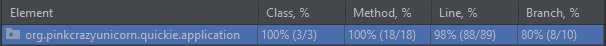
\includegraphics[width=0.98\columnwidth]{Bilder/code-coverage.png}
    \caption{Code Coverage der Applikationsschicht}
    \label{fig:code-coverage}
\end{figure}

\section{Einsatz von Mocks}
\label{sec:mocks}
Mocks spielen eine zentrale Rolle bei der Implementierung von Unit Tests, da sie es ermöglichen, eine Klasse isoliert zu testen. Sie ersetzen dabei die Abhängigkeiten einer Klasse als Objekte mit der für den jeweiligen Test minimal notwendigen Funktionalität. Auch für die im Rahmen dieses Projekts in der Applikationsschicht implementierten Unit Tests kommen Mocks zum Einsatz, welche mit Hilfe des Mocking-Frameworks EasyMock erzeugt werden.

Getestet werden in dieser Schicht der \code{ProfileService} zur Verwaltung der Benutzerprofile, der \code{RecipeService} zur Verwaltung der Rezepte und der \code{MatchingSerivce}, welcher Rezepte mit hoher Übereinstimmung in den Zutaten bestimmt. Alle drei Services besitzen Abhängigkeiten auf mindestens ein Repository für den Zugriff auf Entities und Value Objects. Diese werden für die Unit Tests durch Mocks ersetzt, welche die für den jeweiligen Test notwendigen Daten liefern.
